%%%%%%%%%%%%%%%%%%%%%%%%%%%%%%%%%%%%%%%%%%%%%%%%%%%%%%%%%%%%%%%%%%%%%%%%%%%%%%%%%%%%%%%%%%%%%%%%%%
% Frontiers in Microbiology SUPPLEMENTARY MATERIAL
% Compile separately from the main manuscript (frontiers.tex), using the frontiers_suppmat class.
% Tables and figures are auto-numbered with an "S" prefix (Table S1, Figure S1, ...).
% Do NOT add a title, author list, affiliations, or correspondence in this file.
% Compile on Overleaf/TeX Live: pdflatex x2 (no bibliography needed for this file).
%%%%%%%%%%%%%%%%%%%%%%%%%%%%%%%%%%%%%%%%%%%%%%%%%%%%%%%%%%%%%%%%%%%%%%%%%%%%%%%%%%%%%%%%%%%%%%%%%%

\documentclass[utf8]{frontiers_suppmat}
\usepackage{url,hyperref,lineno,microtype}
\usepackage[onehalfspacing]{setspace}
\graphicspath{{figures/}}
\linenumbers

\begin{document}
\onecolumn
\firstpage{1}

\title {{\helveticaitalic{Supplementary Material}}}

\maketitle

\section{Overview}

This document contains the detailed configuration, provenance, and supporting analyses that
support the main manuscript. It is organized by topic and is numbered independently of the
main text: tables are labelled Table~S1 onward and figures Figure~S1 onward, with the prefix
generated automatically. All items are cited from the main text as Supplementary Table or
Supplementary Figure. The underlying code, configuration files, and full machine-readable
outputs are provided in the reproducibility package and the public repository.

\section{Model architecture and the two training pipelines}

The shared network specification is fixed in \texttt{method\_config.json}, which describes the
layers and feature blocks but contains no training target. Table~\ref{tab:S1} lists the fixed
architecture. The output head depends on the pipeline and is therefore not part of the shared
architecture. Two independent pipeline files specify how the network is trained; their
incompatible settings are contrasted in Table~\ref{tab:S2}. The default contrastive pipeline
uses no classification head and ranks hosts by Euclidean distance, whereas the separate
cross-entropy pipeline adds a full-host softmax head and ranks by logits. Every run record
names the pipeline it used, so the two objectives are never conflated.

\begin{table}[ht]
\centering
\renewcommand{\arraystretch}{1.25}
\caption{Fixed architecture (shared \texttt{method\_config.json}); the output head depends on the pipeline.}\label{tab:S1}
\footnotesize
\begin{tabular}{p{3.1cm} p{11.6cm}}
\hline
Component & Configuration \\
\hline
Input & $1\times64\times64$ FCGR ($k=6$, 4,096 cells); no reverse-complement merge, no pseudocount \\
Convolution 1 & Conv2d(1, 64, k=7, s=2) $\rightarrow 64\times29$; BatchNorm; ReLU \\
Convolution 2 & Conv2d(64, 128, k=7, s=2) $\rightarrow 128\times12$; BatchNorm; ReLU \\
Pooling & MaxPool2d(2) $\rightarrow 128\times6$ \\
Mamba2 block & single bidirectional block; d\_state=128, d\_conv=4, d\_inner=256, 4 heads, chunk=64 \\
Sequence head & flatten 4,608 $\rightarrow$ Linear(512); dropout 0 \\
Coding MLP & 96 $\rightarrow$ 256 $\rightarrow$ 256 $\rightarrow$ 512 \\
Fusion & $(512+128)=640$ $\rightarrow$ Linear(512) $\rightarrow$ ReLU \\
Embedding & 512-d shared output; no head in the contrastive pipeline \\
CE head (CE pipeline only) & Linear(512, n\_candidate\_hosts); full-host softmax \\
\hline
\end{tabular}
\end{table}

\begin{table}[ht]
\centering
\renewcommand{\arraystretch}{1.25}
\caption{The two independent pipelines and their incompatible settings.}\label{tab:S2}
\footnotesize
\begin{tabular}{p{3.3cm} p{5.6cm} p{5.6cm}}
\hline
Setting & Contrastive pipeline (default) & Cross-entropy pipeline \\
\hline
Config file & \texttt{pipeline\_contrastive.json} & \texttt{pipeline\_ce.json} \\
Classification head & none & Linear(512, n\_hosts) \\
Training objective & matrix contrastive loss & softmax cross-entropy \\
Ranking quantity & Euclidean distance (smaller better) & logits (larger better) \\
BN recalibration & 3 passes, momentum=None & not applied \\
Epochs & 120 (100 fusion) & 120 \\
Optimizer & Adam lr=1e-3, no weight decay & Adam lr=1e-3, no weight decay \\
\hline
\end{tabular}
\end{table}

\section{Complete run provenance}

The full provenance file \texttt{full\_provenance.csv} contains one row for each of the 94
runs. Each row records the run identifier, the training script, the pipeline config file, the
split source and its seed, the output JSON, the saved checkpoint, the dataset, the seed, the
train/validation/test sizes, and the test top-1. All 94 checkpoints and every output JSON are
retained. The representative fields in Table~\ref{tab:S3} show the structure of the file;
apparent discrepancies across tables arise from distinct, intentionally different runs rather
than numerical errors.

\begin{table}[ht]
\centering
\renewcommand{\arraystretch}{1.3}
\caption{Provenance structure (the full 94-row file is released; representative fields shown).}\label{tab:S3}
\footnotesize
\begin{tabular}{p{3.6cm} p{2.2cm} p{2.7cm} p{2.7cm} p{2.9cm}}
\hline
Run identifier & Script & Config & Split source & Output / checkpoint \\
\hline
cherry\_random\_cnn\_fcgr\_contrastive\_seed123 & train.py & pipeline\_contrastive.json & random\_split(seed=123) & JSON + .pt both present \\
cherry\_random\_cnn\_mamba\_fcgr\_ce\_seed123 & train.py & pipeline\_ce.json & random\_split(seed=123) & JSON + .pt both present \\
... 92 further runs & train.py / fusion scripts & named per row & random or similarity split & all retained \\
\hline
\end{tabular}
\end{table}

\section{Mash-threshold sensitivity}

The threshold sweep is repeated over three seeds rather than a single seed-123 run. A smaller
Mash threshold is a stricter identity criterion and splits connected components more
aggressively, but it also changes which samples and classes land in the test set rather than
varying one factor in isolation. Table~\ref{tab:S4} reports the multi-seed values and
Figure~\ref{fig:S1} plots the three metrics across thresholds. Because the test composition
changes, this is a descriptive association across partitions, not a controlled dose-response.

\begin{table}[ht]
\centering
\renewcommand{\arraystretch}{1.25}
\caption{Multi-seed Mash-threshold sensitivity (three seeds, mean $\pm$ SD).}\label{tab:S4}
\small
\begin{tabular}{l l l l l}
\hline
Mash threshold & Components & Top-1 & Top-5 & MRR \\
\hline
0.05 & 1,049 & 46.35 $\pm$ 1.11 & 68.09 $\pm$ 2.53 & 56.53 $\pm$ 0.44 \\
0.10 & 807 & 29.59 $\pm$ 2.23 & 53.65 $\pm$ 3.13 & 41.23 $\pm$ 0.54 \\
0.20 & 622 & 26.92 $\pm$ 3.27 & 54.37 $\pm$ 2.95 & 39.79 $\pm$ 2.68 \\
\hline
\end{tabular}
\end{table}

\begin{figure}[ht]
\centering
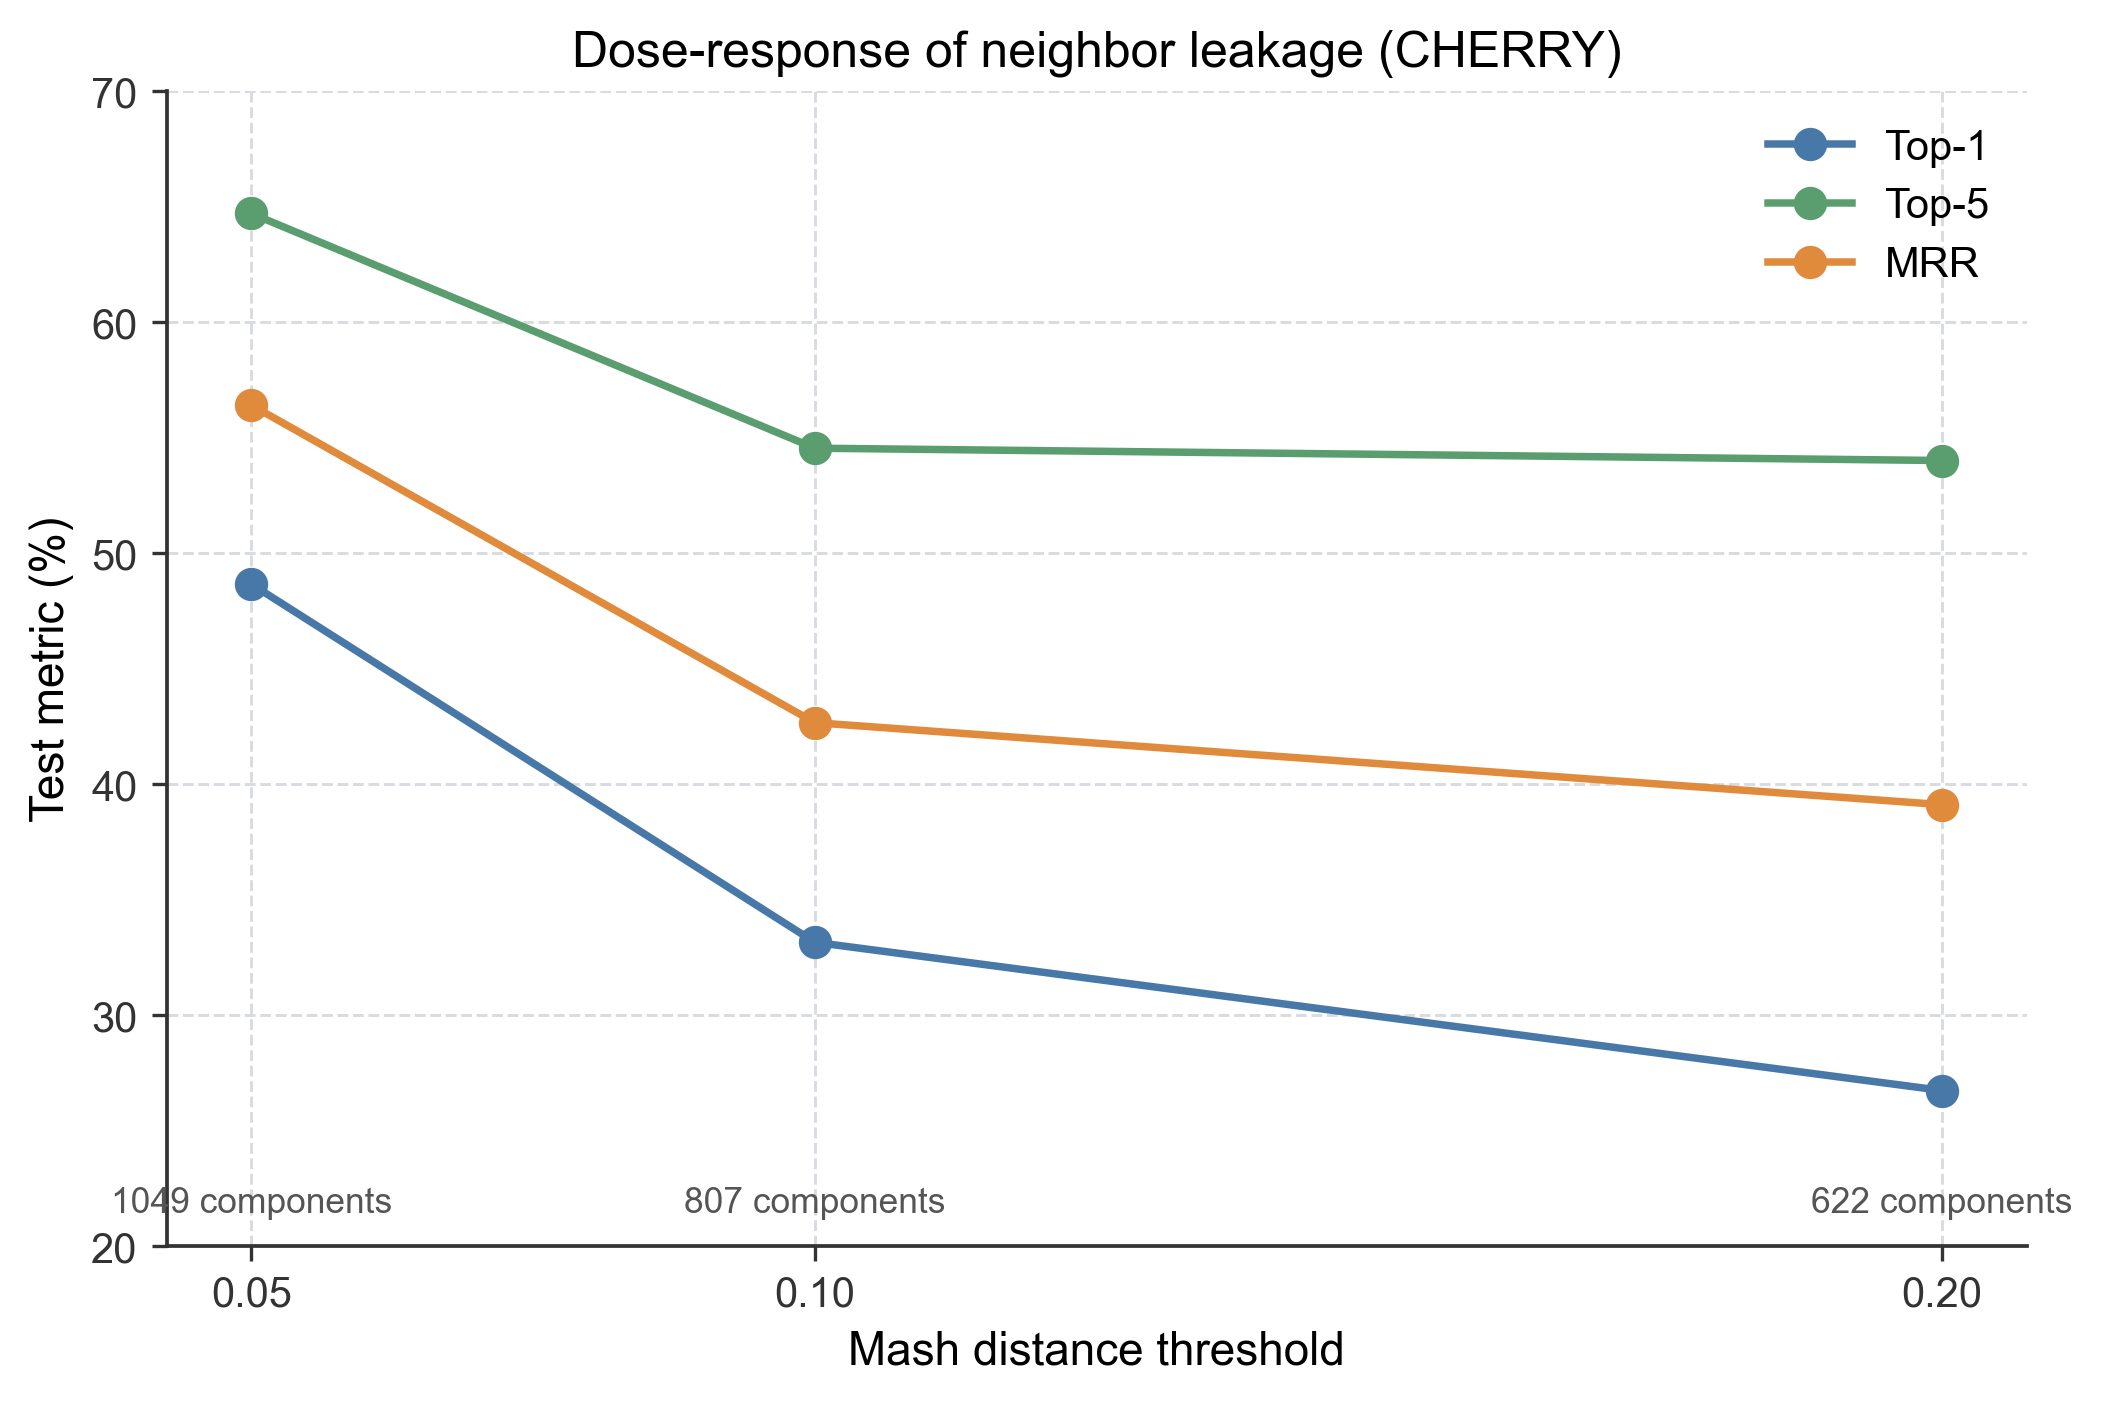
\includegraphics[width=0.85\textwidth]{figS1_threshold.png}
\caption{Top-1, top-5, and MRR across Mash thresholds; each threshold also changes the test composition.}
\label{fig:S1}
\end{figure}

\section{Classical-model tuning sensitivity}

A single uniform validation-set grid is used to test whether the published classical-model
defaults are adequate. Each candidate is trained on the training partition and chosen by
validation top-1, after which the default and the selected model are scored on the same test
set. Table~\ref{tab:S5} is a single-seed, single-split result at seed 123, not a five-seed
mean: the random entries use \texttt{random\_split(seed=123)} and the similarity entries use
\texttt{get\_similarity\_split(seed=123, threshold=0.05)}. The default and tuned models use
identical train/validation/test partitions, so the only thing that changes is the
hyperparameter. The full 32-setting file is released.

\begin{table}[ht]
\centering
\renewcommand{\arraystretch}{1.25}
\caption{Single-seed (seed 123) default versus tuned test top-1 on one fixed split; default and tuned use identical train/validation/test partitions (full 32-setting file released).}\label{tab:S5}
\footnotesize
\begin{tabular}{p{3.6cm} p{3.2cm} l l l}
\hline
Dataset / split / feature & Classifier & Default & Tuned & Change (pp) \\
\hline
CHERRY random FCGR & Logistic regression & 85.14 & 85.71 & +0.57 \\
CHERRY random FCGR & Random forest & 78.86 & 77.14 & $-1.71$ \\
CHERRY random FCGR & K-nearest neighbors & 66.86 & 76.00 & +9.14 \\
CHERRY random FCGR & RBF SVM & 68.57 & 66.86 & $-1.71$ \\
DeepHost random FCGR & Logistic regression & 79.58 & 79.93 & +0.35 \\
DeepHost similarity FCGR & K-nearest neighbors & 43.62 & 53.55 & +9.93 \\
\hline
\end{tabular}
\end{table}

\section{Reference-strain sensitivity}

To test whether the conclusions depend on the chosen reference strain, one species'
representative at a time is replaced with a different strain's RefSeq assembly and the features
and end-to-end predictions are recomputed. The seven species are the best-sampled hosts
spanning different bacterial phyla for which a second, qualifying RefSeq assembly of another
strain exists; an eighth target, \textit{S. viridochromogenes}, had no qualifying second
chromosome-sized record and was excluded. All runs use seed 123, and only the one host under
test is swapped. Table~\ref{tab:S6} reports the feature agreement and the end-to-end change.
The similarity-split flip rate reaches 10.21\% for \textit{E. coli}, which is not described as
negligible, so the conclusion is stated as limited sensitivity with broader strain-level
validation still needed.

\begin{table}[ht]
\centering
\renewcommand{\arraystretch}{1.25}
\caption{Alternative-strain feature agreement and end-to-end change (seven selected species, seed 123).}\label{tab:S6}
\footnotesize
\begin{tabular}{l l l l l}
\hline
Species & FCGR cosine & Protein r & Random flip / delta & Sim. flip / delta \\
\hline
\textit{Escherichia coli} & 0.9991 & 0.99998 & 4.56\% / $-1.05$ & 10.21\% / $-4.93$ \\
\textit{Pseudomonas aeruginosa} & 0.9904 & 0.99666 & 0.00\% / 0.00 & 2.46\% / 0.00 \\
\textit{Salmonella enterica} & 0.9999 & 0.99999 & 0.70\% / +0.35 & 0.00\% / 0.00 \\
\textit{Bacillus cereus} & 0.9695 & 0.99767 & 1.75\% / $-1.05$ & 0.70\% / $-0.70$ \\
\textit{Klebsiella pneumoniae} & 0.9998 & 0.99999 & 0.00\% / 0.00 & 0.00\% / 0.00 \\
\textit{Staphylococcus aureus} & 0.9969 & 0.99888 & 0.70\% / $-0.70$ & 0.00\% / 0.00 \\
\textit{Gordonia terrae} & 0.9947 & 0.99310 & 2.11\% / $-1.40$ & 1.41\% / $-1.06$ \\
\hline
\end{tabular}
\end{table}

\section{Host-phylogeny controls}

The phylogeny controls separate the part of the codon signal that operates at the genus level
from the part that survives control for shared ancestry. The genus-level, genus-mean, and
within-genus analyses use the real genus label and are post-hoc diagnostics, not deployable
prediction inputs; the host-tree principal components are learned without labels.
Table~\ref{tab:S7} reports the controls. Genus-mean residualization causes a large decline,
showing that a substantial component of the signal is shared at the genus rank, while
within-genus discrimination remains high and host-tree PC residualization changes accuracy
only slightly.

\begin{table}[ht]
\centering
\renewcommand{\arraystretch}{1.25}
\caption{Host-phylogeny controls (top-1; random five-seed mean, similarity seed 123).}\label{tab:S7}
\footnotesize
\begin{tabular}{l l l l l}
\hline
Control & CHERRY random & CHERRY sim. & DeepHost random & DeepHost sim. \\
\hline
Species codon baseline & 77.98 & 54.01 & 82.88 & 63.38 \\
Genus-level prediction & 85.43 & 70.05 & 88.98 & 71.48 \\
Genus-mean residualized & 30.85 & 15.51 & 28.42 & 14.79 \\
Host-tree PC residualized & 74.36 & 52.41 & 82.18 & 56.69 \\
Within-genus discrimination & 85.75 & 68.07 & 88.94 & 79.17 \\
\hline
\end{tabular}
\end{table}

\section{DeepHost within-dataset replication}

The same within-dataset patterns recur on DeepHost, where the coding encoder again exceeds
FCGR with a larger margin after leakage control. Table~\ref{tab:S8} reports the three
representation variants over five seeds with uncertainty for every metric.

\begin{table}[ht]
\centering
\renewcommand{\arraystretch}{1.25}
\caption{DeepHost within-dataset replication over five seeds (mean $\pm$ SD for every metric).}\label{tab:S8}
\footnotesize
\begin{tabular}{l l l l l}
\hline
Variant / split & Top-1 & Top-5 & MRR & Macro-F1 \\
\hline
FCGR / random & 80.91 $\pm$ 2.17 & 90.53 $\pm$ 1.24 & 85.36 $\pm$ 1.80 & 55.06 $\pm$ 3.29 \\
Coding / random & 83.44 $\pm$ 2.80 & 92.84 $\pm$ 1.44 & 87.72 $\pm$ 1.89 & 62.11 $\pm$ 3.57 \\
Fusion / random & 84.00 $\pm$ 2.19 & 93.54 $\pm$ 1.83 & 88.17 $\pm$ 1.50 & 61.53 $\pm$ 3.76 \\
FCGR / similarity & 54.30 $\pm$ 1.04 & 73.38 $\pm$ 2.15 & 63.45 $\pm$ 1.09 & 31.89 $\pm$ 3.11 \\
Coding / similarity & 63.52 $\pm$ 1.55 & 82.25 $\pm$ 2.51 & 71.89 $\pm$ 1.06 & 40.21 $\pm$ 1.38 \\
Fusion / similarity & 62.96 $\pm$ 1.52 & 80.49 $\pm$ 2.75 & 70.96 $\pm$ 1.44 & 39.16 $\pm$ 2.90 \\
\hline
\end{tabular}
\end{table}

\section{Coding sub-block ablation}

The sub-block ablation identifies codon frequencies as the strongest single block, reaching
50.98\% under the similarity split on its own, close to the full encoder; the amino-acid block
is next and the structural block weakest. Table~\ref{tab:S9} reports the block-level results and
Figure~\ref{fig:S2} presents them with seed variability.

\begin{table}[ht]
\centering
\renewcommand{\arraystretch}{1.25}
\caption{Coding sub-block ablation (top-1, three-seed mean).}\label{tab:S9}
\small
\begin{tabular}{l l l}
\hline
Feature block & Random & Similarity \\
\hline
Structure only (8) & 58.51 & 27.63 \\
Codon only (64) & 76.77 & 50.98 \\
Amino-acid + physicochemical (24) & 74.65 & 44.39 \\
Codon + amino-acid (88) & 79.08 & 53.12 \\
\hline
\end{tabular}
\end{table}

\begin{figure}[ht]
\centering
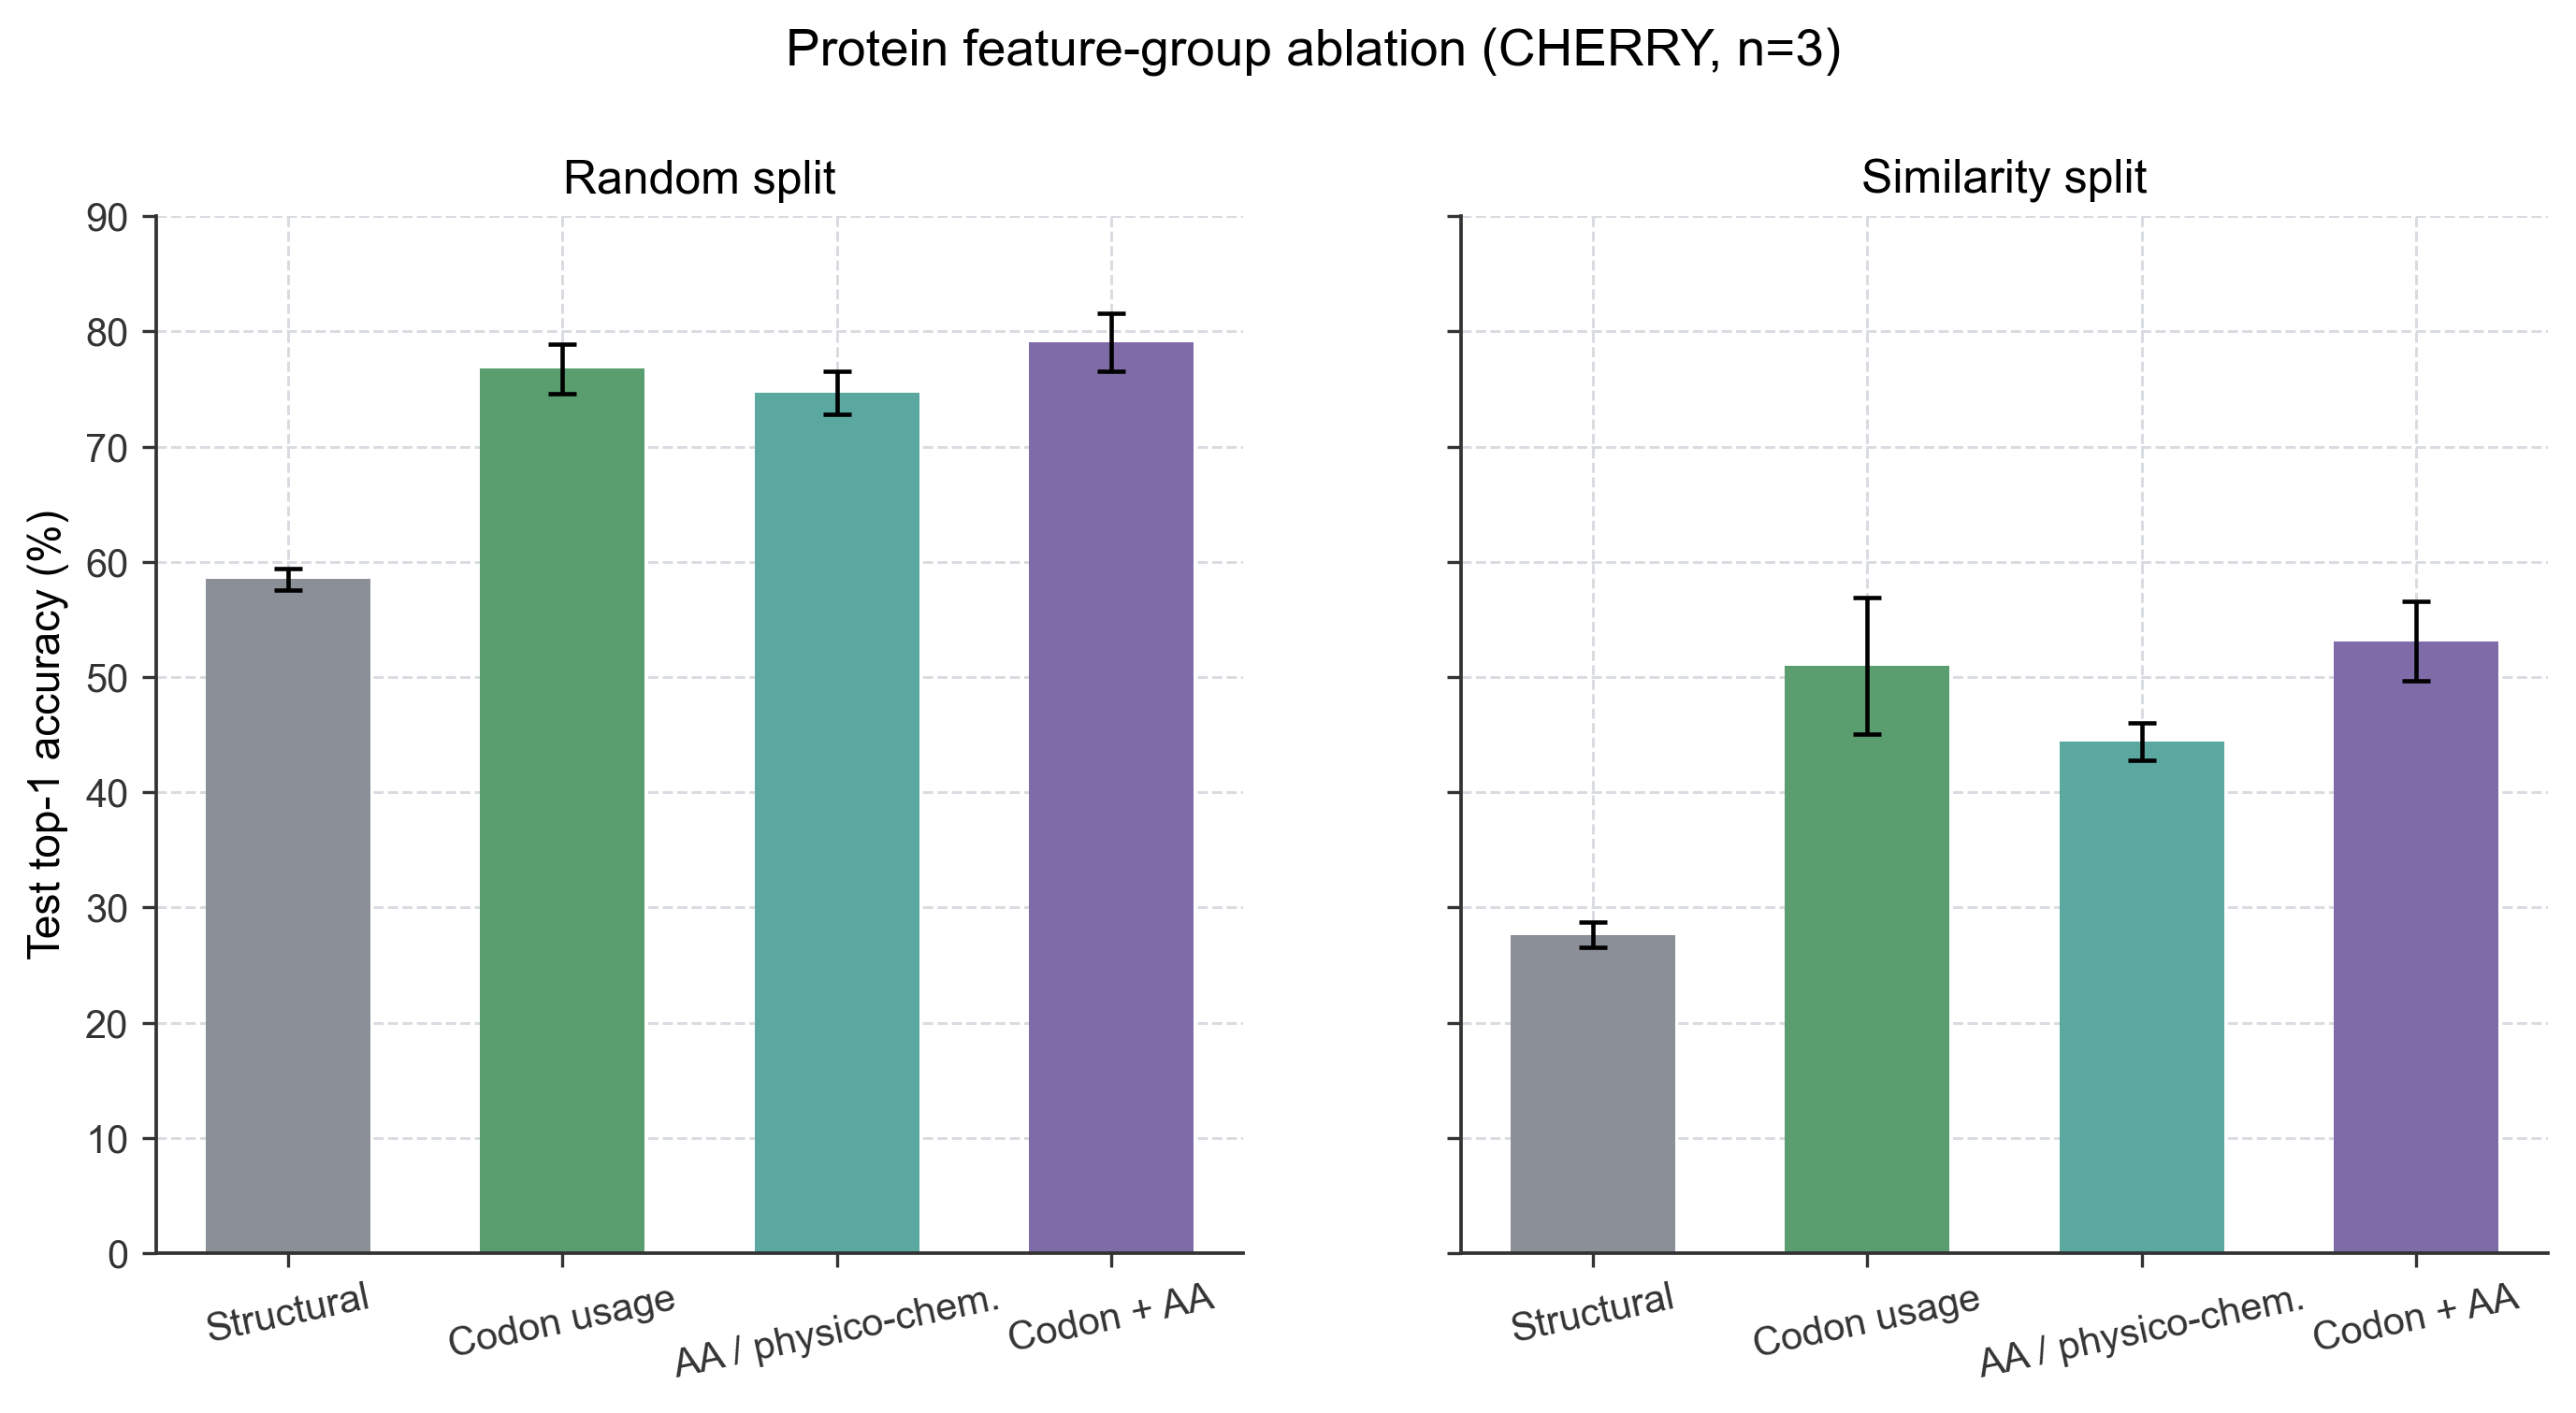
\includegraphics[width=0.85\textwidth]{figS2_ablation.png}
\caption{Coding sub-block ablation (three-seed mean $\pm$ SD) under the random and similarity splits.}
\label{fig:S2}
\end{figure}

\section{Inference efficiency}

The efficiency protocol is run on an NVIDIA RTX 4090 (CUDA 12.4, FP32, batch 32, 10 warm-up
and 100 timed iterations over five repeats, GPU-synchronized, forward only). Table~\ref{tab:S10}
reports parameter counts and latency. The full model uses 3.07 million parameters and
$2.52\pm0.02$ ms per batch, the CNN-only variant 2.76 million and 0.24 ms, and PhageCGRNet
67.4 million and 2.68 ms.

\begin{table}[ht]
\centering
\renewcommand{\arraystretch}{1.25}
\caption{Parameter count and inference latency under the documented forward-only protocol (five repeats).}\label{tab:S10}
\small
\begin{tabular}{l l l}
\hline
Model & Parameters & Latency per batch (ms) \\
\hline
BMKMPHI full & 3,066,520 & 2.522 $\pm$ 0.017 \\
CNN-only variant & 2,764,928 & 0.241 $\pm$ 0.003 \\
PhageCGRNet & 67,424,846 & 2.679 $\pm$ 0.022 \\
\hline
\end{tabular}
\end{table}

\section{Full per-class recall}

The full per-class recall distribution complements the main-text imbalance analysis.
Figure~\ref{fig:S3} shows the CHERRY per-class recall across all 65 evaluated classes, of which
32 have zero recall with mean recall 0.473. Figure~\ref{fig:S4} shows the DeepHost per-class
recall across 65 classes, of which 19 have zero recall with mean recall 0.636.

\begin{figure}[ht]
\centering
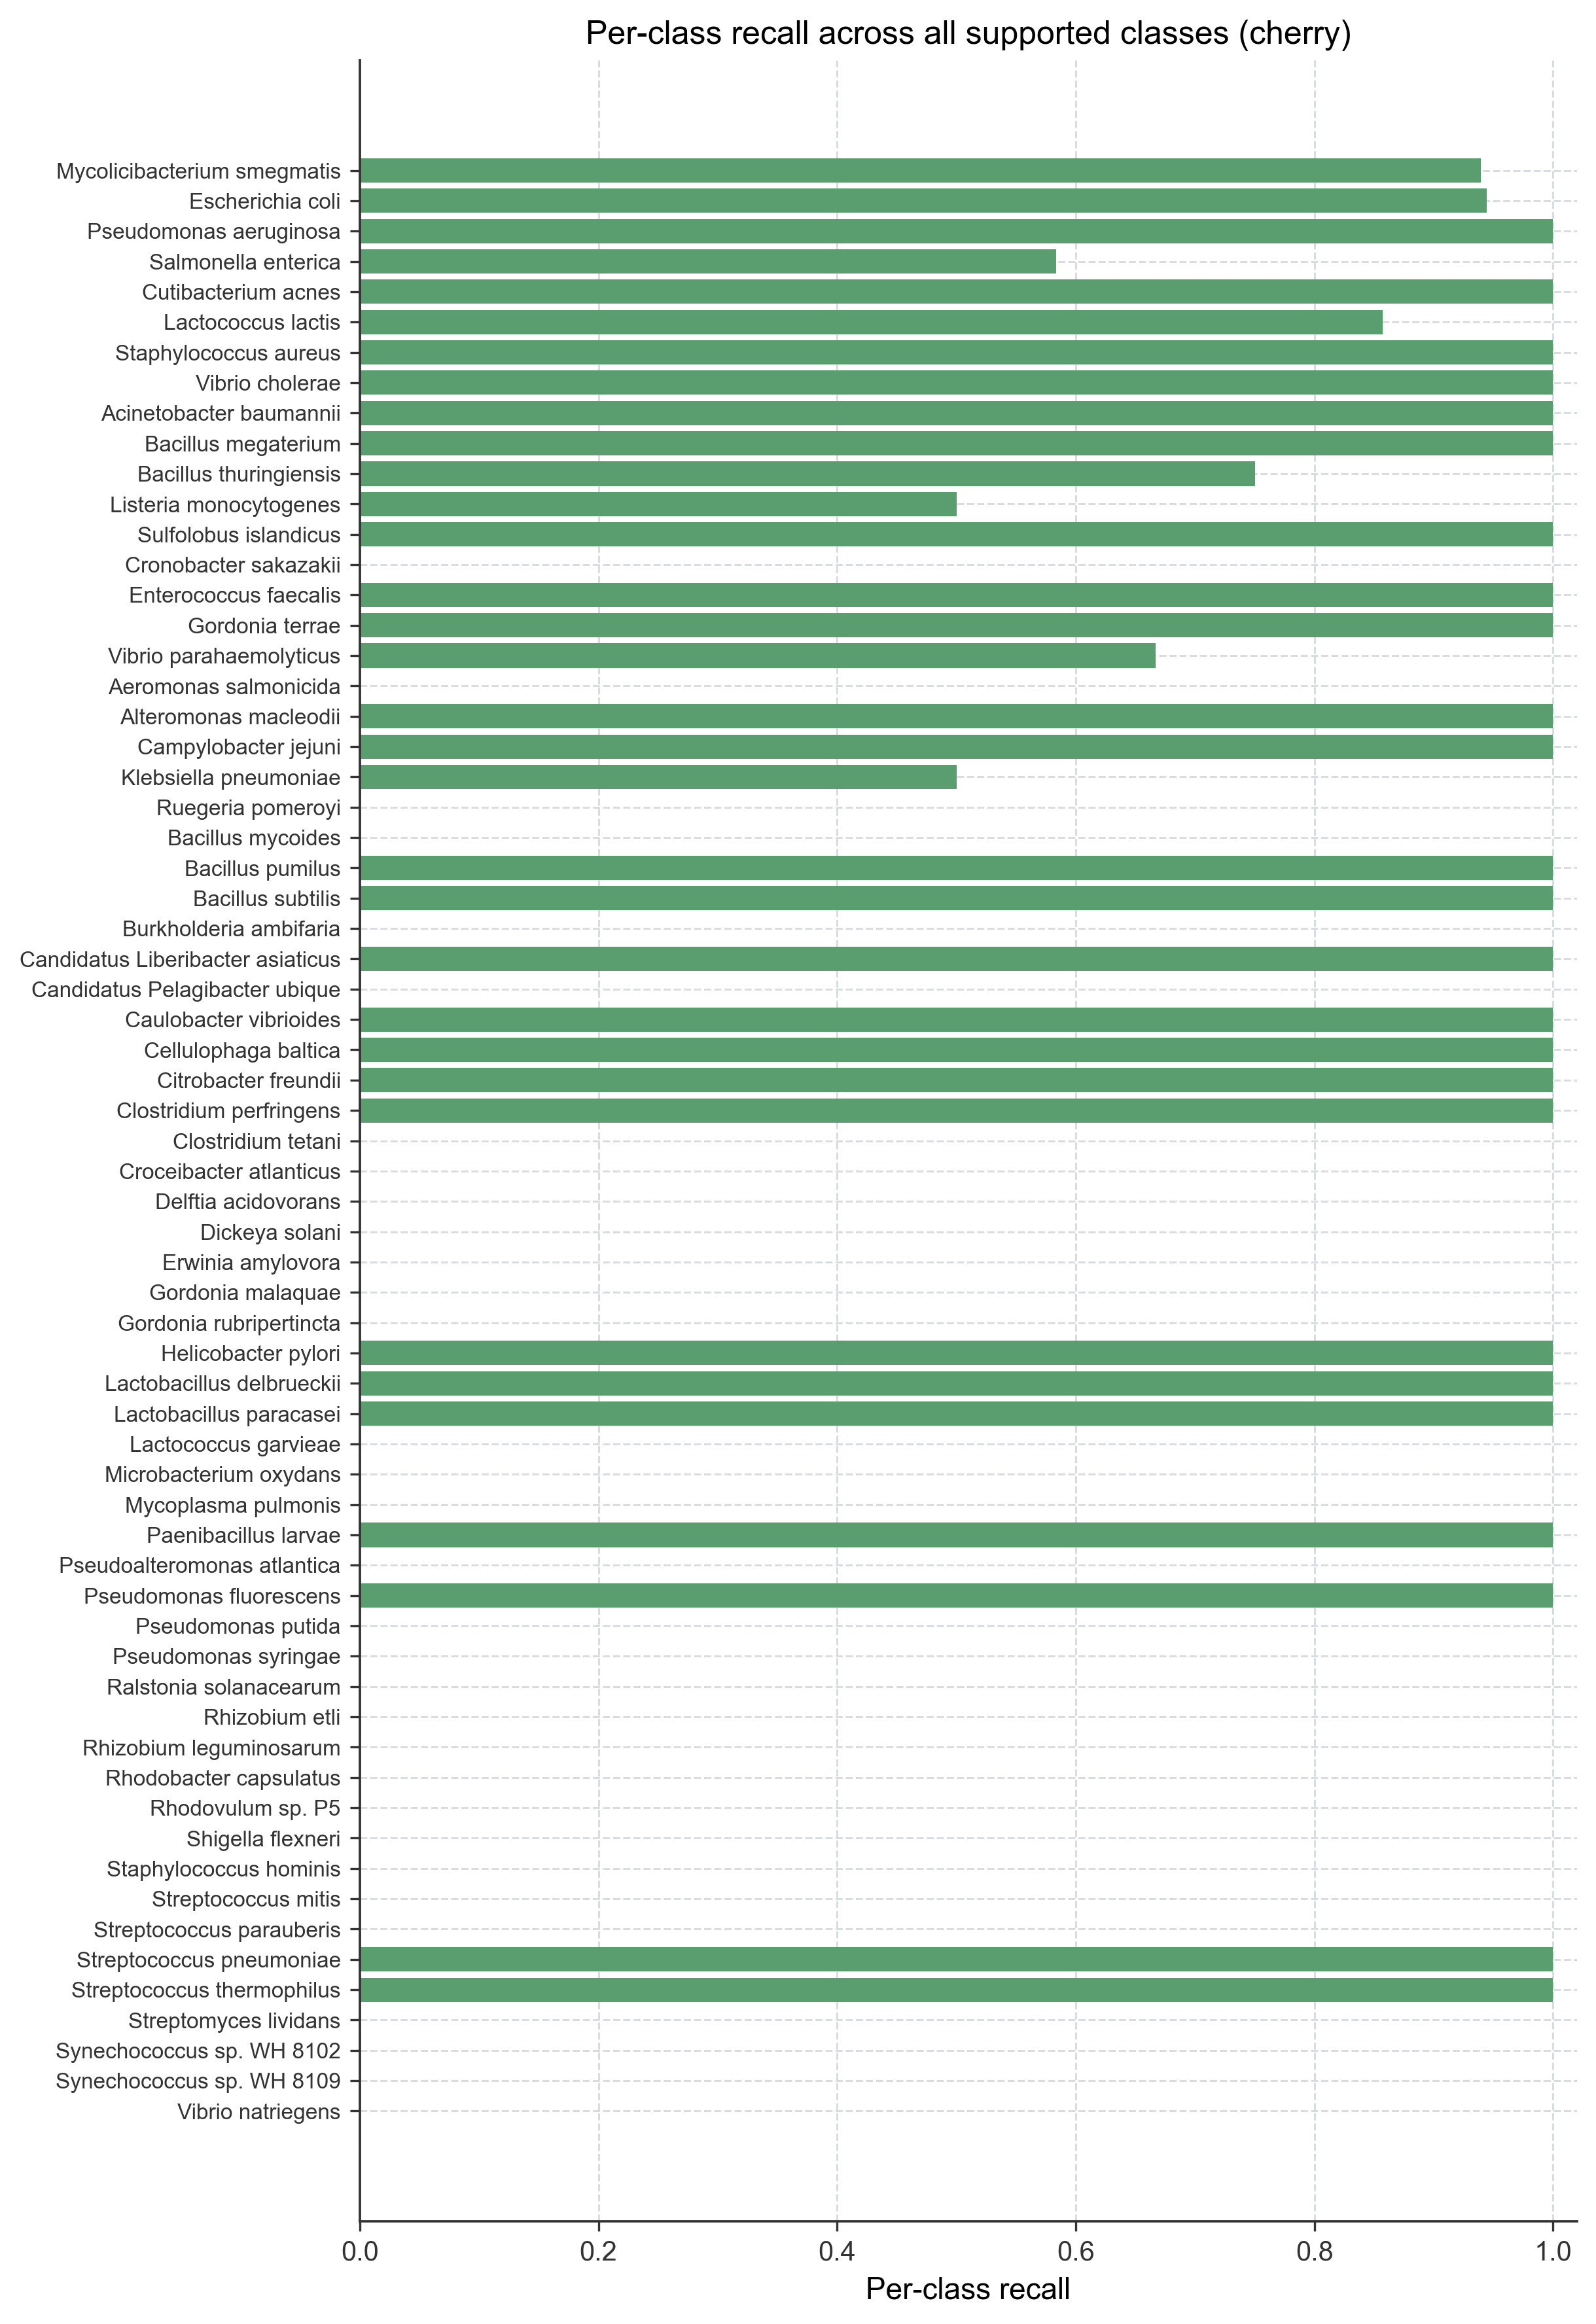
\includegraphics[width=0.95\textwidth]{figS3_recall_cherry.png}
\caption{Per-class recall across all evaluated CHERRY classes (65); 32 classes have zero recall and the mean per-class recall is 0.473.}
\label{fig:S3}
\end{figure}

\begin{figure}[ht]
\centering
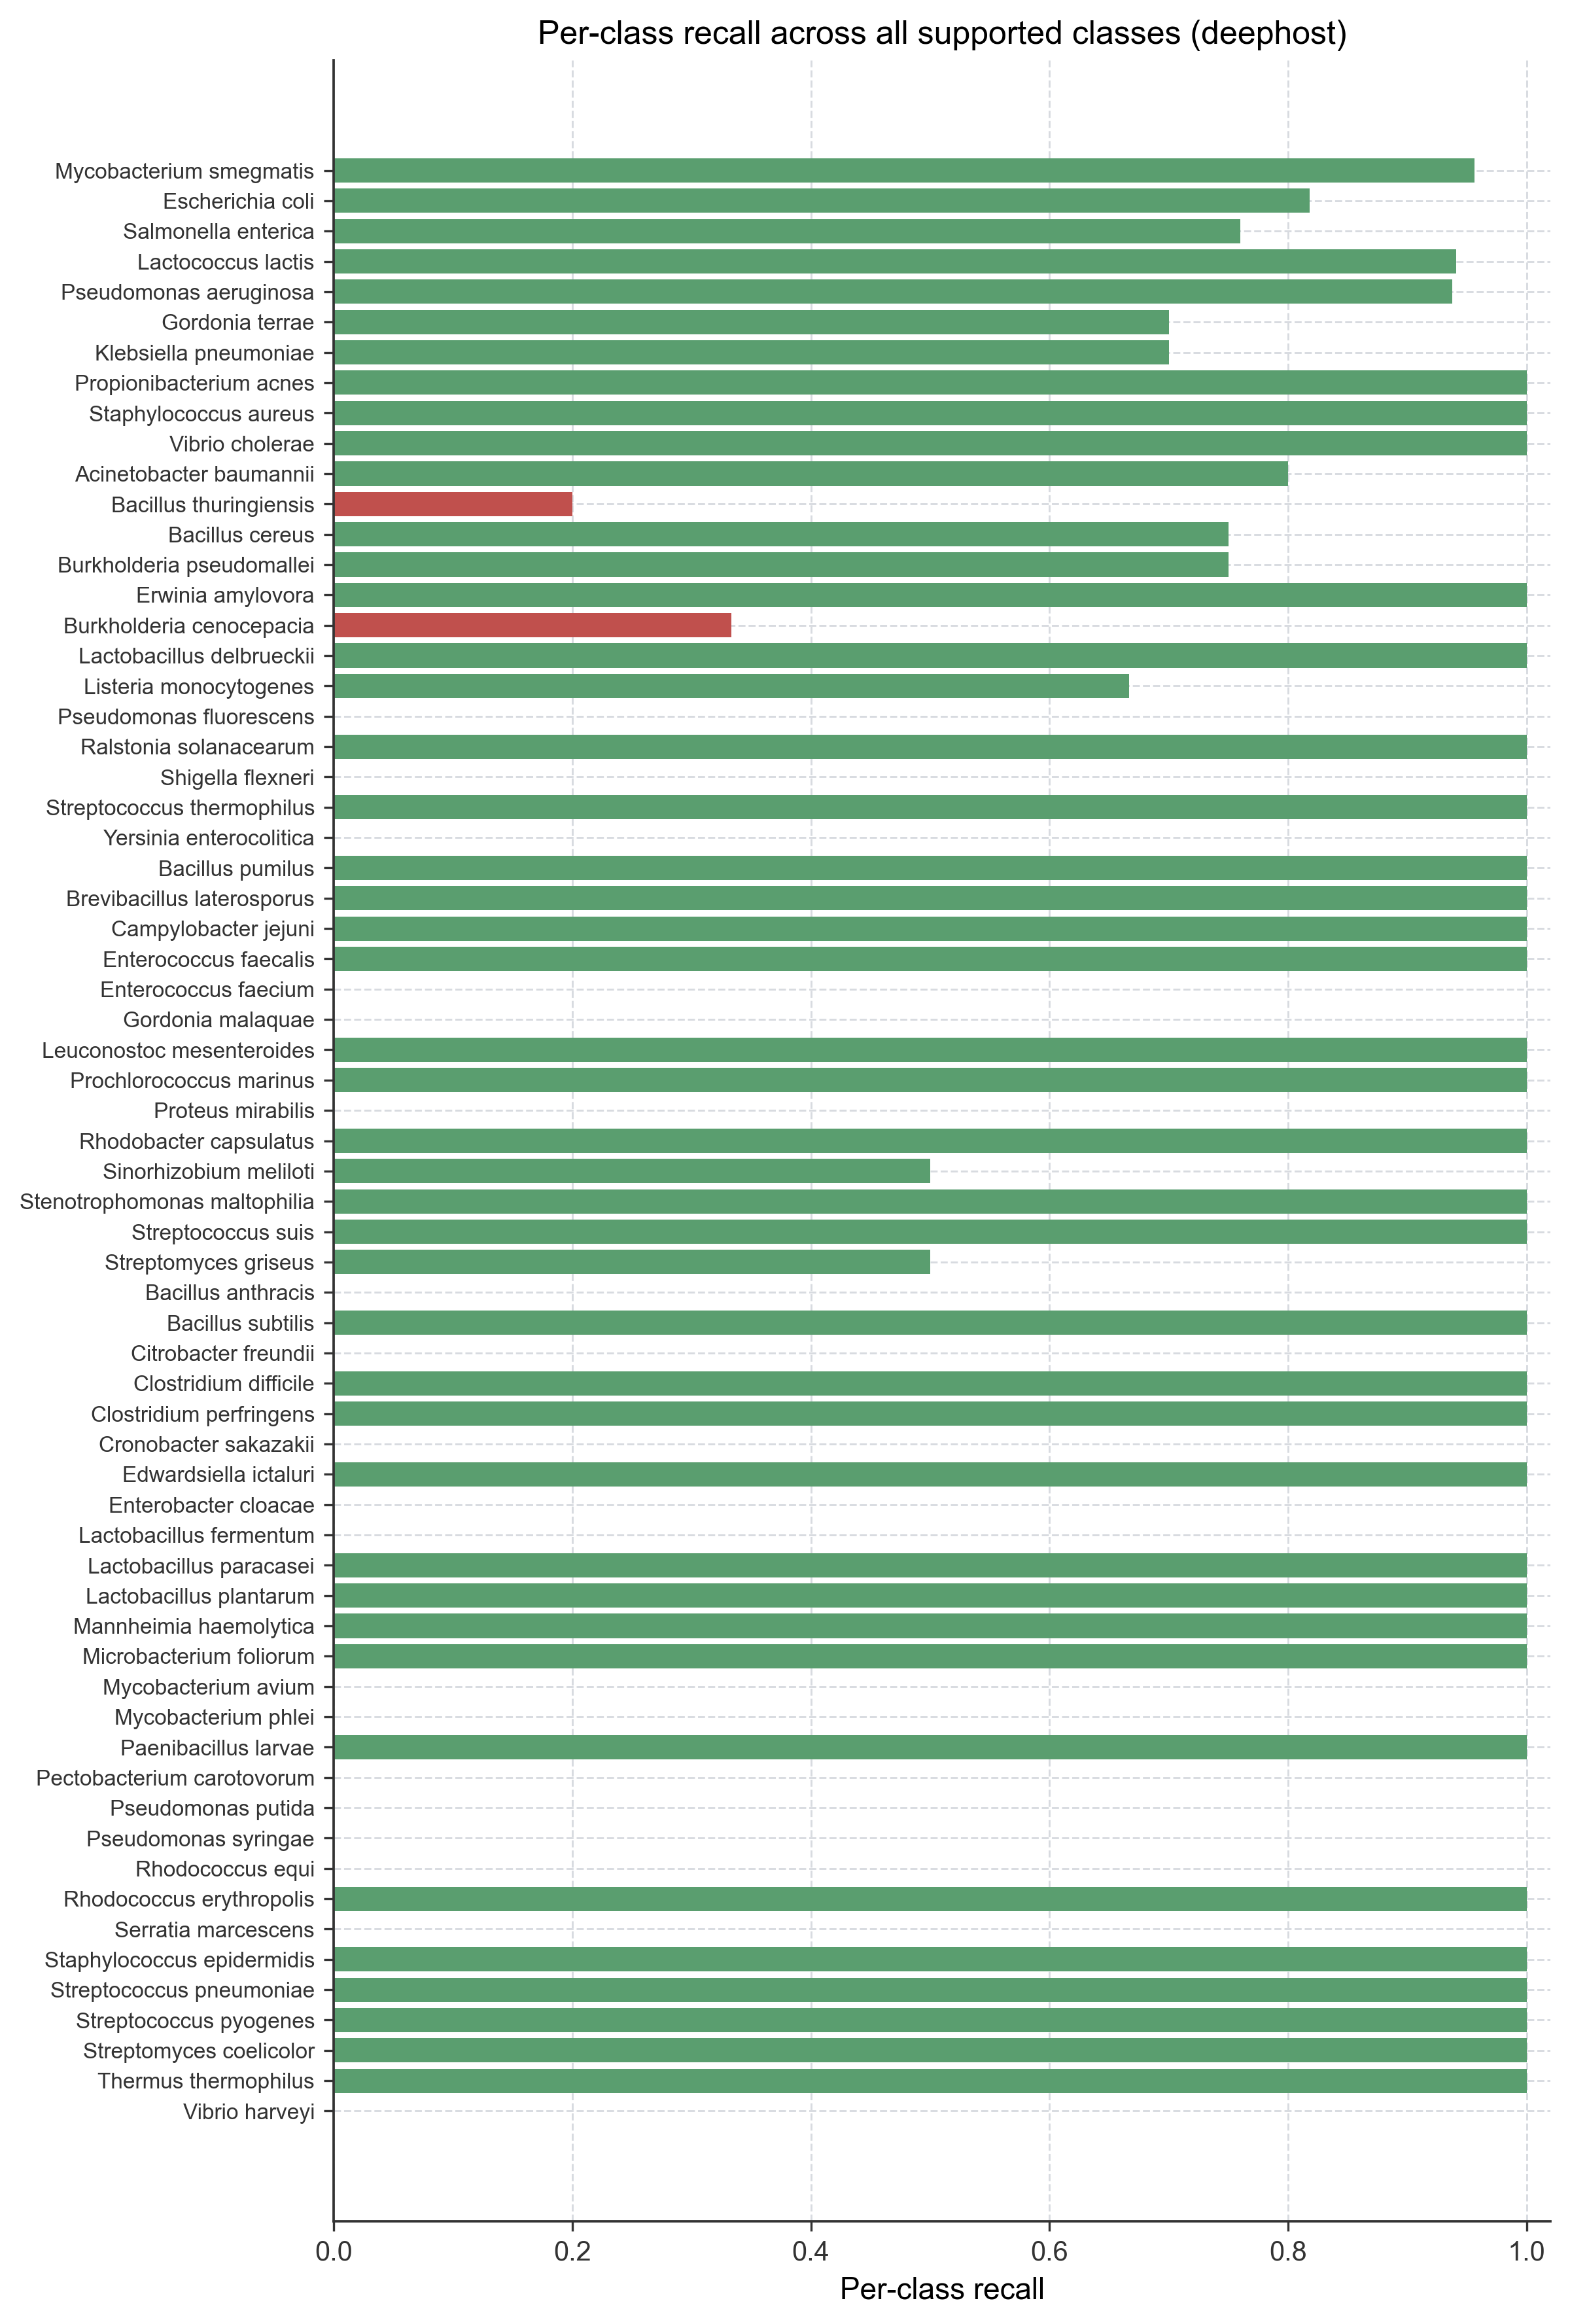
\includegraphics[width=0.95\textwidth]{figS4_recall_deephost.png}
\caption{Per-class recall across all evaluated DeepHost classes (65); 19 classes have zero recall and the mean per-class recall is 0.636.}
\label{fig:S4}
\end{figure}

\end{document}
